\documentclass[../main-report.tex]{subfiles}
\begin{document}
\section{Vấn đề đặt ra}
\label{sec:problem}
Hoạt động từ thiện là một hoạt động được đông đảo mọi người quan tâm, theo kết quả của một cuộc khảo sát \cite{vuhongphong_tuthien} cho thấy có tới 81\% người ở nước ta được khảo sát cho rằng những hoạt động tình nguyện thì họ rất quan tâm đến. Tương tự có khoảng 83\% cho rằng hoạt động từ thiện đặc biệt quan trọng đối với một đất nước đang phát triển như Việt Nam.

Tuy nhiên, các hoạt động từ thiện thì chưa được đông đảo người dân thực sự tin tưởng. Thật vậy, trong một cuộc khảo sát \cite{asiafoundation_thuthien} có hơn 50\% người dân thành thị (người dân thành thị chiếm đa số trong nguồn gây quỹ) cho rằng các hoạt động từ thiện của người dân hiện tại chưa công khai minh bạch, và đứng sau đó là các lý do được thể hiện ở hình \ref{fig:chart-problem-charity1} như: chưa tạo niềm tin, chưa đúng đối tượng, chưa tuyên truyền tốt, thiếu nguồn lực.

\begin{figure}[ht!]
\begin{center}
\label{fig:chart-problem-charity1}
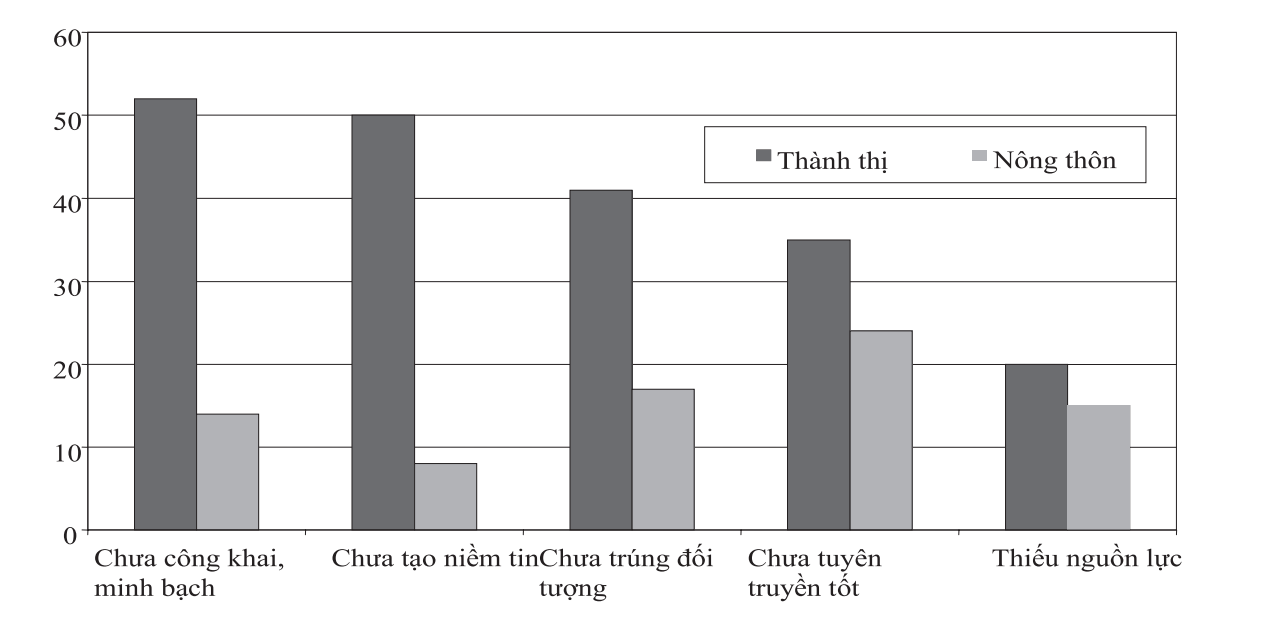
\includegraphics[scale=0.65]{chart-problem-charity1}
\caption{Những lý do chưa tạo được niềm tin trong hoạt động từ thiện của người dân}
\end{center}
\end{figure}

Đối với các hoạt động từ thiện của các doanh nghiệp, cũng trong cuộc khảo sát trên thì có tới hơn 50\% người dân thành phố Hồ Chí Minh cho rằng lý do khiến họ không tin tưởng vào hoạt động từ thiện của doanh nghiệp là chưa đúng đối tượng cần được hỗ trợ. Lý do này chiếm tỉ lệ cao nhất trong các lý do được liệt kê ở hình \ref{fig:chart-problem-charity2}.

\begin{figure}[ht!]
\begin{center}
\label{fig:chart-problem-charity2}
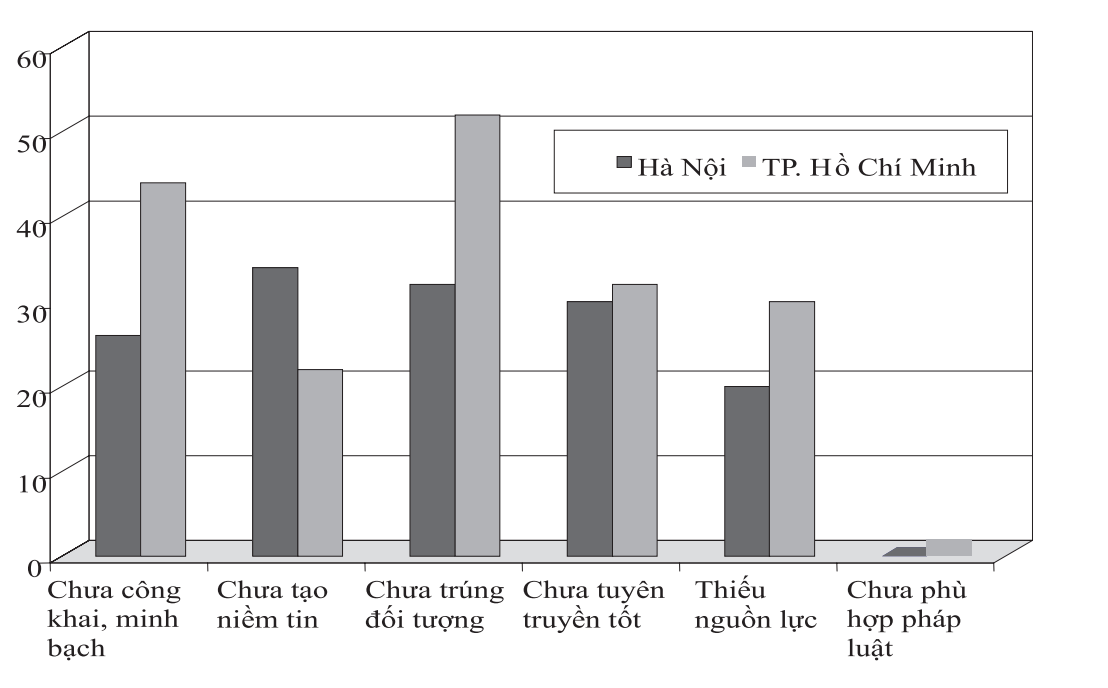
\includegraphics[scale=0.65]{chart-problem-charity2}
\caption{Những lý do chưa tạo được niềm tin trong hoạt động từ thiện của doanh nghiệp}
\end{center}
\end{figure}

Trong một bài nghiên cứu về từ thiện của tác giả Bekkers và Wiepking \cite{bekkers2011literature}, các cá nhân sẽ đóng góp từ thiện nếu họ 
\begin{enumerate*}[label=(\roman*)]
\item nhận thức được nhu cầu của người cần giúp đỡ, ví dụ như biết cụ thể người cần giúp đỡ;
\item được vận động đóng góp bởi một tổ chức đáng tin cậy;
\item nhận thấy chi phí cho việc đóng góp (thuế) nhỏ và lợi ích khi đóng góp rõ ràng;
\item động cơ nhân ái mạnh mẽ;
\item nhận thấy việc đóng góp từ thiện có lợi cho danh tiếng bản thân;
\item nhận thấy lợi ích về mặt tâm lý, ví dụ như thoải mái khi đem cho;
\item đóng góp cho những giá trị sống vì cộng đồng, và
\item thấy rõ tính hiệu quả.
\end{enumerate*}

Trong sách trắng của nền tảng Alice\footnote{https://alice.si} cũng chỉ ra rằng sự minh bạch trong các hoạt động gây quỹ từ thiện ở các nước trên thế giới khiến cho lòng tin người dân sụt giảm một cách đáng kể. \cite{alice}

Do đó việc tạo ra một ứng dụng gây quỹ từ thiện theo mô hình gây quỹ cộng đồng áp dụng công nghệ \gls{blockchain} là cần thiết. Ứng dụng có thể loại bỏ sự kiểm soát về mặt tài chính của các tổ chức, các giao dịch được công khai, minh bạch và đảm bảo được chiến dịch là đáng tin cậy khi nó được xác minh bởi tổ chức, cơ quan chuyên trách.

\section{Tính khoa học và tính mới của đề tài}
\subsection{Tính khoa học}
Với các vấn đề đặt ra ở phần \ref{sec:problem}, hệ thống mà nhóm tác giả xây dựng sẽ:

\begin{itemize}
\item Giải quyết vấn đề công khai, minh bạch trong hoạt động gây quỹ khi xây dựng mô hình ứng dụng phi tập trung bằng công nghệ \gls{blockchain}.
\item Loại bỏ sự kiểm soát tài chính bởi các tổ chức, thay vào đó là ứng dụng hợp đồng thông minh trong công nghệ \gls{blockchain} để phân bổ dòng tiền một cách tự động và an toàn.
\item Tăng cường niềm tin ở người đóng góp quỹ khi các chiến dịch được xác minh một cách công khai trước khi đưa đến cộng đồng mà không tiết lộ các thông tin liên quan tới quyền riêng tư bằng công nghệ mã hoá.
\item Tạo ra những cuộc bỏ phiếu của người đóng góp quỹ cho việc phân bổ nguồn quỹ một cách công khai, minh bạch bằng hợp đồng thông minh. Do đó tăng cường quyền hạn của người đóng góp quỹ.
\end{itemize}

\subsection{Tính mới}
\begin{itemize}
\item Xây dựng ứng dụng gây quỹ từ thiện theo mô hình gây quỹ cộng đồng.
\item Ứng dụng công nghệ \gls{blockchain} vào hoạt động gây quỹ từ thiện.
\item Xây dựng ứng dụng với các tính năng nổi bật so với các ứng dụng hiện tại như: hoàn tiền tự động khi chiến dịch gây quỹ không đạt được mục tiêu, lưu trữ và quản lý thông tin định danh người dùng, giải ngân và bỏ phiếu giải ngân theo nhiều giai đoạn.
\end{itemize}

\section{Mục tiêu}
Mục tiêu khi thực hiện khóa luận này bao gồm:

\begin{itemize}
\item Xây dựng một ứng dụng web gây quỹ cộng đồng cho mục đích từ thiện dựa trên công nghệ \Gls{blockchain} để tăng cường tính minh bạch, công khai với các chức năng cơ bản: lập hồ sơ gây quỹ, vận động gây quỹ, đóng góp tiền vào chiến dịch gây quỹ, phân phối tiền gây quỹ.
\item Tạo cơ chế để ứng dụng đảm bảo các yêu cầu sau:
\begin{itemize}
\item Các chiến dịch gây quỹ phải được xác minh trước khi công khai cho những người đóng góp.
\item Đảm bảo nguồn quỹ được chuyển trực tiếp từ người đóng góp tới người thụ hưởng.
\item Nguồn quỹ chỉ được phân phối theo lộ trình nếu như mục tiêu đặt ra trong hồ sơ gây quỹ được hoàn thành và được những người ủng hộ chấp nhận bằng cách bỏ phiếu.
\end{itemize}
\end{itemize}

\section{Đối tượng nghiên cứu}
Thứ nhất về mặt công nghệ, tập trung nghiên cứu nền tảng công nghệ Ethereum và hợp đồng thông minh.

Thứ hai về mặt nghiệp vụ, nghiên cứu các phương thức gây quỹ từ thiện bằng tài chính, các quy trình, giai đoạn của hoạt động gây quỹ.

\section{Phạm vi nghiên cứu}
Khóa luận tập trung vào nghiên cứu các chiến dịch gây quỹ từ thiện cộng đồng bằng internet, các chiến dịch gây quỹ với người tạo chiến dịch có am hiểu về công nghệ blockchain và đồng tiền mã hóa.
\end{document}